\section{Related Work}
\label{sec:related_work}
%\vspace{-5pt}
%We review the most relevant work in 3D reconstruction that aligns with our contribution, focusing on neural surface reconstruction, generalizable neural radiance fields, and Gaussian splatting techniques.
\vspace{-5pt}
\noindent{\bf Neural Surface Reconstruction}
Neural implicit representations have significantly advanced neural surface reconstruction by modeling 3D geometries as continuous functions computable at any spatial location. These methods offer compact and efficient ways to capture complex shapes, demonstrating strong performance in 3D reconstruction \cite{darmon2022improving, jiang2020sdfdiff, kellnhofer2021neural, niemeyer2020differentiable, oechsle2021unisurf, wang2021neus, yariv2021volume, yariv2020multiview, yu2022monosdf}, shape representation \cite{atzmon2020sal, gropp2020implicit, mescheder2019occupancy, park2019deepsdf}, and novel view synthesis \cite{liu2020neural, mildenhall2021nerf, trevithick2021grf}. The introduction of NeRF \cite{mildenhall2021nerf} marked a significant shift, leading to further advancements. For instance, IDR \cite{yariv2020multiview} uses multi-view images for surface rendering but requires object masks. Variants of NeRF, such as those incorporating Signed Distance Functions (SDF), have shown promising results in geometry reconstruction. NeuS \cite{wang2021neus} presents an unbiased volumetric weight function with logistic sigmoid functions, while Volsdf \cite{yariv2021volume} integrates SDF into density formulation with a sampling strategy to maintain error bounds. HF-NeuS \cite{wang2022hf} improves NeuS by modeling transparency as a transformation of the signed distance field and using a coarse-to-fine strategy to refine high-frequency details.
Over-fitting, especially in the few-shot setting, can be alleviated with regularization (smoothness priors \eg \cite{niemeyer2021regnerf,kim2022infonerf,robust,ntps}, adversarial priors \eg \cite{dro,nap,sparseocc,augnerf}, additional modalities \eg \cite{rgbd,sparsecraft,deng2021depth,wang2023sparsenerf}) or data priors.
Despite their effectiveness, these methods often require extensive optimization and a high volume of dense images, posing challenges for generalization and scalability.\\
%\vspace{-10pt}
\noindent{\bf Generalizable Neural Radiance Fields and Surface Reconstruction}
Recent advancements in neural radiance fields (NeRFs) have improved novel view synthesis from sparse observations by exploring various strategies for scene geometry \cite{deng2022depth, niemeyer2022regnerf, wynn2023diffusionerf, jain2021putting, kim2022infonerf}. Pose estimation approaches like NeRF-Pose \cite{nerfpose} and NeRF-Feat\cite{nerfeat} perform surface reconstruction implicitly to render feature images and correspondence images in contrast to depth estimation task. Generalizable methods harness data priors for reconstruction from images and point clouds (\eg \cite{p2s,nksr,poco,fssdf,mixing}) to produce occupancy, SDF, radiance and light fields (\eg \cite{lfn,lfnr,genlf}).   
Techniques such as \cite{chen2021mvsnerf, johari2022geonerf, chibane2021stereo, liu2022neural, wang2021ibrnet, yu2021pixelnerf} extend NeRFs to novel scenarios using priors from multi-view datasets.
% Recent advancements in neural radiance fields (NeRFs) have improved novel view synthesis from sparse observations by exploring various strategies for scene geometry \cite{deng2022depth, niemeyer2022regnerf, wynn2023diffusionerf, jain2021putting, kim2022infonerf}. Techniques such as \cite{chen2021mvsnerf, johari2022geonerf, chibane2021stereo, liu2022neural, wang2021ibrnet, yu2021pixelnerf} extend NeRFs to novel scenarios using priors from multi-view datasets.
For example, PixelNeRF \cite{yu2021pixelnerf} and MVSNeRF \cite{chen2021mvsnerf} utilize CNN features and warped image features, respectively. However, achieving accurate scene geometry with NeRF-based methods can be challenging due to density threshold tuning issues, as noted in Unisurf \cite{oechsle2021unisurf}. Recent progress includes integrating NeRFs with Signed Distance Function (SDF) techniques to model volume density effectively. Methods such as SparseNeuS \cite{long2022sparseneus} and VolRecon \cite{ren2023volrecon} leverage image priors, with SparseNeuS using a regular volume rendering and VolRecon incorporating multi-view features through a transformer. ReTR \cite{liang2024retr} and UfoRecon \cite{na2024uforecon} employ advanced transformers for feature extraction and cross-view matching. GeoTransfer \cite{jena2024geotransfer} finetunes a pretrained SOTA NeRF to learn accurate occupancy fields. Despite these advances, volumetric rendering frameworks often result in slow rendering speeds, hindering real-time performance.

\begin{figure*}[t!] % h = here, t = top, b = bottom, p = page
    %\centering
    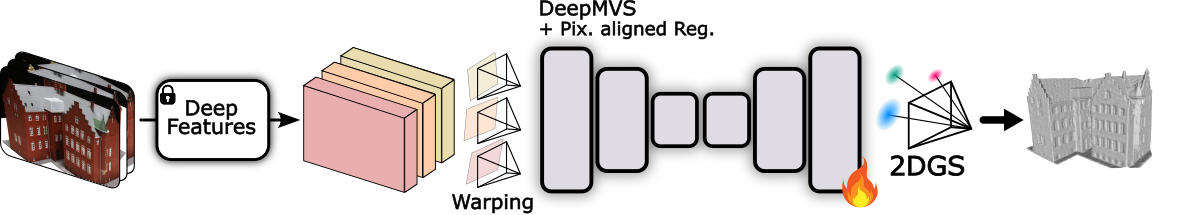
\includegraphics[width=1.05\textwidth]{figs/pipeline} % Change to your image file
    \caption{We present the first generalizable feed-forward 2DGS prediction model from multi-view images. It achieves state-of-the-art performance in the sparse DTU \cite{aanaes2016large} 3D reconstruction benchmark \cite{long2022sparseneus}, with faster inference by several orders of magnitude compared to the competition based on volume rendering of implicit representations. Multi-view input deep features are homography-warped into the target view. A two-fold network performs Deep Multi-view Stereo and pixel aligned 2D surface element attribute regression. Perspective accurate Gaussian Splatting \cite{huang20242d} of these surface elements enables real-time novel view synthesis and mesh extraction.}
    \label{fig:pipe}
\end{figure*}

%\vspace{-12pt}
\noindent{\bf Gaussian Splatting}
Explicit representations combined with neural rendering 
\cite{aliev2020neural,jena2022neural,dnr,fvs}
have had considerable success previously albeit with an important computational cost. 3D (3DGS) \cite{kerbl20233d} and 2D Gaussian Splatting (2DGS) \cite{huang20242d} employ anisotropic Gaussians for explicit scene representation, enabling real-time rendering through differentiable rasterization. 2DGS improves view consistency and depth map quality by reducing one scaling dimension. This technique has been applied to various domains, including scene editing \cite{Gaussianeditor, cen2023saga}, dynamic scenes \cite{yang2023deformable3dgs, luiten2023dynamic, wu20234dgaussians}, and avatars \cite{GauHuman, GaussianAvatar, 3DGS-Avatar}. Despite its effectiveness, Gaussian Splatting often overfits specific scenes. Recent approaches \cite{pixelsplat, chen2024mvsplat} aim to generalize Gaussian Splatting for unseen scenes by predicting Gaussian parameters in a feed-forward manner, avoiding per-scene optimization. PixelSplat \cite{pixelsplat} addresses scale ambiguity using an epipolar Transformer, although it incurs high computational costs, while MVSplat \cite{chen2024mvsplat} builds a cost volume representation via plane sweeping, reducing learning difficulty and enabling faster, lightweight models. However, these methods face limitations related to object reconstruction scope and specific input configurations. Our approach introduces a more efficient and generalizable method for 3D reconstruction and novel view synthesis across diverse, unseen scenes by leveraging the MVS backbone of MVSGaussian \cite{liu2024fast}, which combines Multi-View Stereo for encoding geometry-aware Gaussian representations with hybrid Gaussian and volume rendering for improved generalization and real-time performance. Differently from \cite{liu2024fast}, we use the 2DGS representation as it benefits the consistency of our 3D geometry.  
We further utilize robust monocular as well as multi-view features from the foundation models (DinoV2 \cite{oquab2023dinov2} and MASt3R \cite{leroy2024grounding}) to improve the generalizability of our approach. Our method achieves state-of-the-art results in 3D reconstruction and novel view synthesis with faster inference compared to previous generalizable implicit 3D reconstruction approaches. We note that while our method uses MASt3R within a feed-forward pipeline, concurrent work such as InstantSplat \cite{instsplat} and Sparfels \cite{sparfels} propose to use it in a test-time optimization scenario.  


